\chapter{Collaboration in Immersive Virtual Environment - A General State of the Art}
\label{chapter:context}
\minitoc

\section{Introduction}
This chapter presents a general state of the art of different topics related to using immersive virtual environment for collaborative task. Being the joint interest of Virtual Reality (VR) and Computer Supported Collaborative Work (CSCW).

With rapid increasing computation capacity and the development of computer network, multi-agent collaboration via computer-generated virtual space with new types of communication and interaction becomes available.

\section{Virtual Reality}
\subsection{Definition}
Virtual reality related devices appeared before the term itself was created. The \textit{Sensorama Machine} invented in 1957 and patented in 1962 by Morton Heiling believes to be the first multi-sensorial application (Figure~\ref{fig:1_earlyapp}-left). It is a simulator which provides the illusion of reality using a 3-D motion picture with smell, stereo sound, vibrations of the seat, and wind in the hair to create the illusion \footnote{http://www.mortonheilig.com/InventorVR.html}. Then in 1968, Ivan Sutherland with the help of his student Bob Sproull created the first virtual reality and augmented reality (partly see-through) headset named ``The Sword of Damocles" \citep{Sutherland1968Hmd} (Figure~\ref{fig:1_earlyapp}-right).

\begin{figure}[htb]
  \centering
  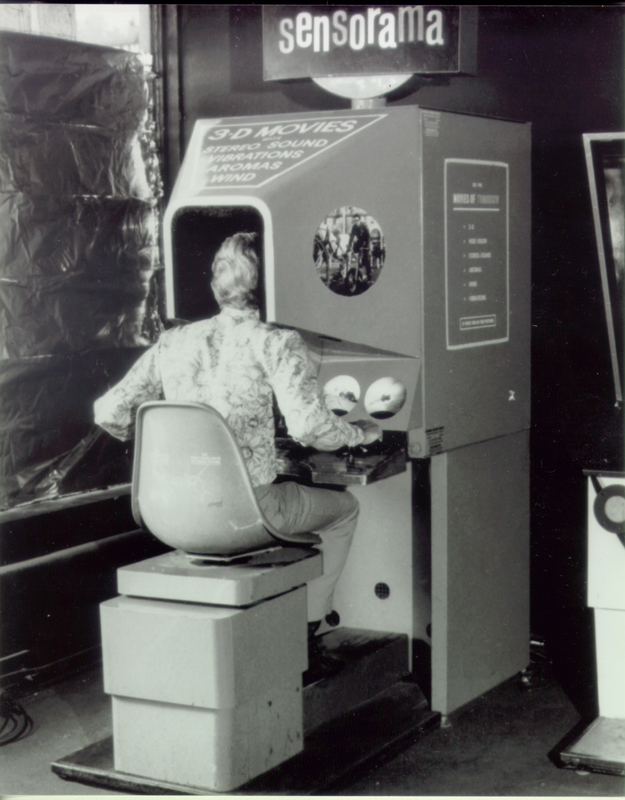
\includegraphics[height=7.5cm]{figures/ch1/sensorama}
  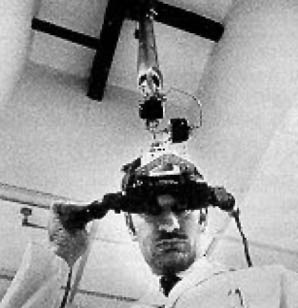
\includegraphics[height=7.5cm]{figures/ch1/ultimateHMD}
  \caption{\label{fig:1_earlyapp}First virtual reality applications: Sensorama Machine (left); The first head mounted display (right).}
\end{figure}

The term ``Virtual reality" in its modern usage was coined and popularized by Jaron Lanier \citep{Lanier1992VR} through his company VPL Research in 1980's. Early definitions of virtual reality are often device-oriented which refer to a certain type of sophisticated computer equipment serving as a medium to connect users to a digitally created space. In the meanwhile, researchers began to discuss and establish conceptual framework of virtual reality, switching from device-oriented definitions to user experience based understanding. Especially, the term ``presnece" or ``telepresence" was introduced to describe the generic perception of being in an artificial environment \citep{Sheridan1992MTV}, which is one of the key notions of VR and will be discussed more thoroughly later on. More elaborated discussions about the history and definition of virtual reality can be found in \citet{Rheingold1991VR}'s book and \citet{Steuer1995Defining}'s paper.

Nowadays, a relatively complete definition of virtual reality was given by another book of \citet{Fuchs2011Book}: ``Virtual reality is a scientific and technical domain that uses computer science and behavioral interfaces to simulate in a virtual world the behavior of 3D entities, which interact in real time with each other and with one or more users in pseudo-natural immersion via sensorimotor channels."

This definition covers three important aspects of virtual reality:

First, virtual reality is both a technical and scientific domain. On one hand, technological progress makes unthinkable experiences become available and provides a hardware platform on which theoretical research of virtual reality is based. For example, CAVE and Head-Mounted Display bring a higher level of visual immersion so that users can actually ``step in" the virtual world and have the sensation of ``being at another place". Real-time tracking devices like leap motion and kinect enable motion capture so that users can interact with computers using natural gestures and other types of body movement. On the other hand, researchers make further investigations of the cause and influencing factors of user's subjective feelings using existing devices, and in return, provide guidelines for the development of future virtual reality systems.

Virtual reality is an extension of human computer interaction (HCI) as we move from traditional desktop to 3D user interface, many of its research methods are inherited or inspired by HCI research work. However, unlike HCI which is design-oriented and tries to find efficient, ergonomic and aesthetic interfaces for interaction, virtual reality aims to ``remove" this interface and let users interact naturally with the virtual world. Virtual reality groups research efforts from various domains as it relies on different technical science domains (e.g. computer science, robotics and automatics etc.) and also on contributions from human and behavioral science (e.g. cognitive psychology, physiology, neurobiology, etc.).

Second, virtual reality possesses two key characteristics which distinguish itself with other existing technologies related to 3D virtual environment: sensorial immersion and real time interaction. In desktop or console based video games, players enjoy real time interaction in the virtual world alone or with other players. They use input devices like joystick, mouse and keyboard which offers very limited sensorial immersion. On the contrary, 3D movies projected on large screens in the cinema give the audience good visual immersion, but no interaction capability. The emergence of virtual reality technology brings great changes to the way we are connected to the virtual world. Having the feeling of being immersed in another world and being able to interact in real time in that world as naturally as in the real world is quite appealing and may change completely the game and movie industries. Of course, the application of virtual reality technology is not limited to these domains, it also has great impact on education, product design, training, etc. Here is a summary of virtual reality applications (ref TODO).

Last and the most important, it reveals three main components of virtual reality system: the virtual environment, the user, and the behavioral interface allowing them to interact. The ``perception, decision and action" loop \citep{Fuchs2011Book} describes how users interact with the surrounding virtual world, which is a transposition of the ``perception, cognition, action" loop demonstrating man's behavior in a real world. As shown in Figure~\ref{fig:1_loop}, the user acts (vocal commands, gestures and other body movements, etc.) on the virtual environment through motor interfaces, and these activities are captured and transferred to the computer system. Then the computer system makes corresponding changes to the virtual environment and generates sensorial reactions (images, sound, haptic, etc.) which are transferred to the user via sensorial interfaces.

\begin{figure}[htb]
  \centering
  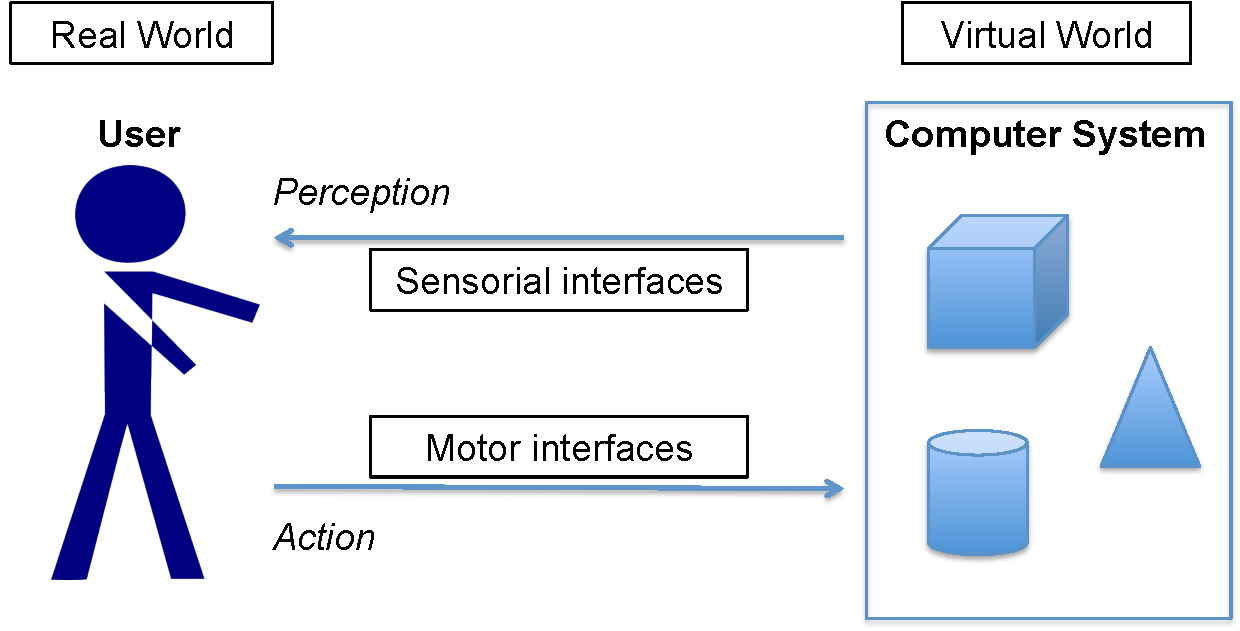
\includegraphics[width=0.9\textwidth]{figures/ch1/loop}
  \caption{\label{fig:1_loop}The ``perception, decision and action" loop in interactive virtual environment.}
\end{figure}

Since the virtual world is totally generated by the computer system, two inherent issues need to be solved: the latency and the sensorimotor discrepancies. The latency is the time lag between the user's action on motor interfaces and the perception of the consequences of this action on the virtual environment through sensorial interfaces. This artifact influences every virtual reality application and may be the source of many problems related to user comfort. The sensorimotor discrepancies is another problem for virtual reality applications. With technical progression, we can simulate more complex phenomenons and provide more interaction through sensorimotor interfaces in the virtual environment, but the real world offers way more information for us to simulate with current technology and the sensorimotor discrepancies will continue to exist.

Now we will discuss in more details about the three components of virtual reality system mentioned above: the virtual environment, the behavioral interfaces and the human inside.

\subsection{Virtual Environment}
Virtual environment is a term often used to describe computer-generated synthetic space, similar to virtual world. However, more strictly speaking, as \citet{Ellis1991VE} explained, an environment is the theater of human activity, so virtual environment is a human-centered notion, not only refers to an artificial world model. For example, according to \citet{Fox2009Guide}: ``A virtual environment is a digital space in which a user's movements are tracked and his or her surroundings rendered, or digitally composed and displayed to the senses, in accordance with those movements." This definition emphasizes that a virtual environment is a virtual space that can react to user's movements and change accordingly.

\citet{Ellis1991VE} summarized three parts which form a virtual environment: content, geometry and dynamics. The content is often organized as scene graph with clear hierarchical structure and inter relationship between objects. Each object possesses a state vector containing properties such as position, orientation, velocity and color, etc. The geometry is a description of an environmental field of action which has dimensionality, metrics and extent, and the dynamics of an environment are the rules of interaction among its contents describing their behavior, such as physical laws (gravity, object collision, etc.). More details on the description of virtual environment can be found in \citet{Ellis1991Pictorial}'s book.

In virtual reality applications, the diversity of origins of the worlds represented in the virtual environment makes virtual reality more than a simple copy of the ``reality" that we live in. As summarized by \citet{Fuchs2011Book}, the virtual world could be a simulation of certain aspects of the real world, but also a completely symbolic or imaginary world. The visual representation of of objects could vary depending on our need, and spatial, temporal and physical laws may or may not be applied in the virtual world. For example, we can visualize and interact with structure of molecules, flow of fluids under different scales \citep{Ferey2009Multisensory, Bryson1996Virtual}, we can also change the speed of light to better visualize and understand phenomenons of relativity \citep{Doat2011NRP}, or the entire world could just be a figment of imagination of an artist or a science-fiction writer.


\subsection{Behavioral Interfaces}
As mentioned in \citet{Fuchs2011Book}'s definition of virtual reality, behavioral interface is a term to describe a type of interfaces that connect the user to the virtual environment. Unlike traditional human computer interfaces which act as a communication tool (e.g. keyboard), behavioral interfaces use the motricity or perceptions of man resulting from his/her behavior in the real world to carry out activities in a virtual world. As shown in Figure~\ref{fig:1_loop}, two types of behavioral interface exist: sensorial interfaces are designed to transfer sensory stimuli from computer to the user while the motor interfaces transfer motor responses from the user to the computer, thus we can also call them sensorimotor interfaces. One of the current challenges of virtual reality is to build more efficient and transparent interfaces based on human sensory channels and motor activities.

\subsubsection{Visual Interface}
As the idiom ``Seeing is believing" states, the visual sense is nearly the most important sensory channel that humans use to discover the real world, which is also true in virtual reality applications. The software and hardware advancements in computer graphics constantly improve the quality of real time three-dimensional images, which allows more complex and photo-realistic rendering. The display used as visual interface should have the following characteristics:

\begin{itemize}
\item Large field of view (FoV) both in horizontal and vertical directions (``borderless").
\item Stereoscopic vision in the entire binocular field of vision.
\item High graphic resolution (pixel density), currently most widely used is 1080p FullHD display, but displays with higher resolution are on the way.
\item Head or eye tracking compatible. Since we can move our head and eyes to look into different directions, it is necessary to assure that user always has perspective-correct view of the virtual scene. This can be achieved by using tracking devices\footnote{see section \ref{sec:tracking}.}
\end{itemize}

A lot of display systems exist nowadays which satisfy all or part of the characteristics listed above, from large immersive rooms and wall displays to table-sized screen, and even portable screens mounted on user's head (see Figure~\ref{fig:1_vi}). They vary in size, form, display technology and aimed applications. Only CAVE (Figure~\ref{fig:1_vi:cave}) and HMD (Figure~\ref{fig:1_vi:hmd}) are designed to provide fully visual immersion. Other displays, on the contrary, can not assure a user to always stay visually inside the virtual world, but they can offer good visual immersion and are better suited for data visualization and 3D object interaction in certain cases. There are also some special display solutions not mentioned above that can provide individual stereoscopic views of 3D models such as the volumetric display \citep{Grossman2008Volum} and holographic display \citep{Lucente1997Holo}, but currently they can only be applied to non-immersive context with even smaller workspace.


\begin{figure}[htb]
  \begin{subfigure}{.3\textwidth}
    \centering
    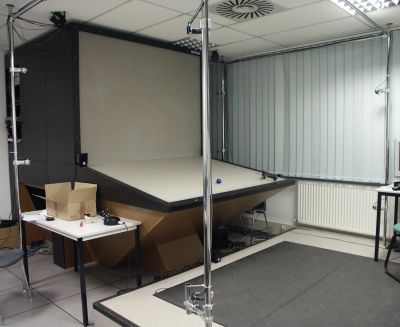
\includegraphics[height=3.5cm]{figures/ch1/workbench}
    \caption{Workbench formed by two separate screens (LIRIS-CNRS).}
    \label{fig:1_vi:bench}
  \end{subfigure}
  \begin{subfigure}{.3\textwidth}
    \centering
    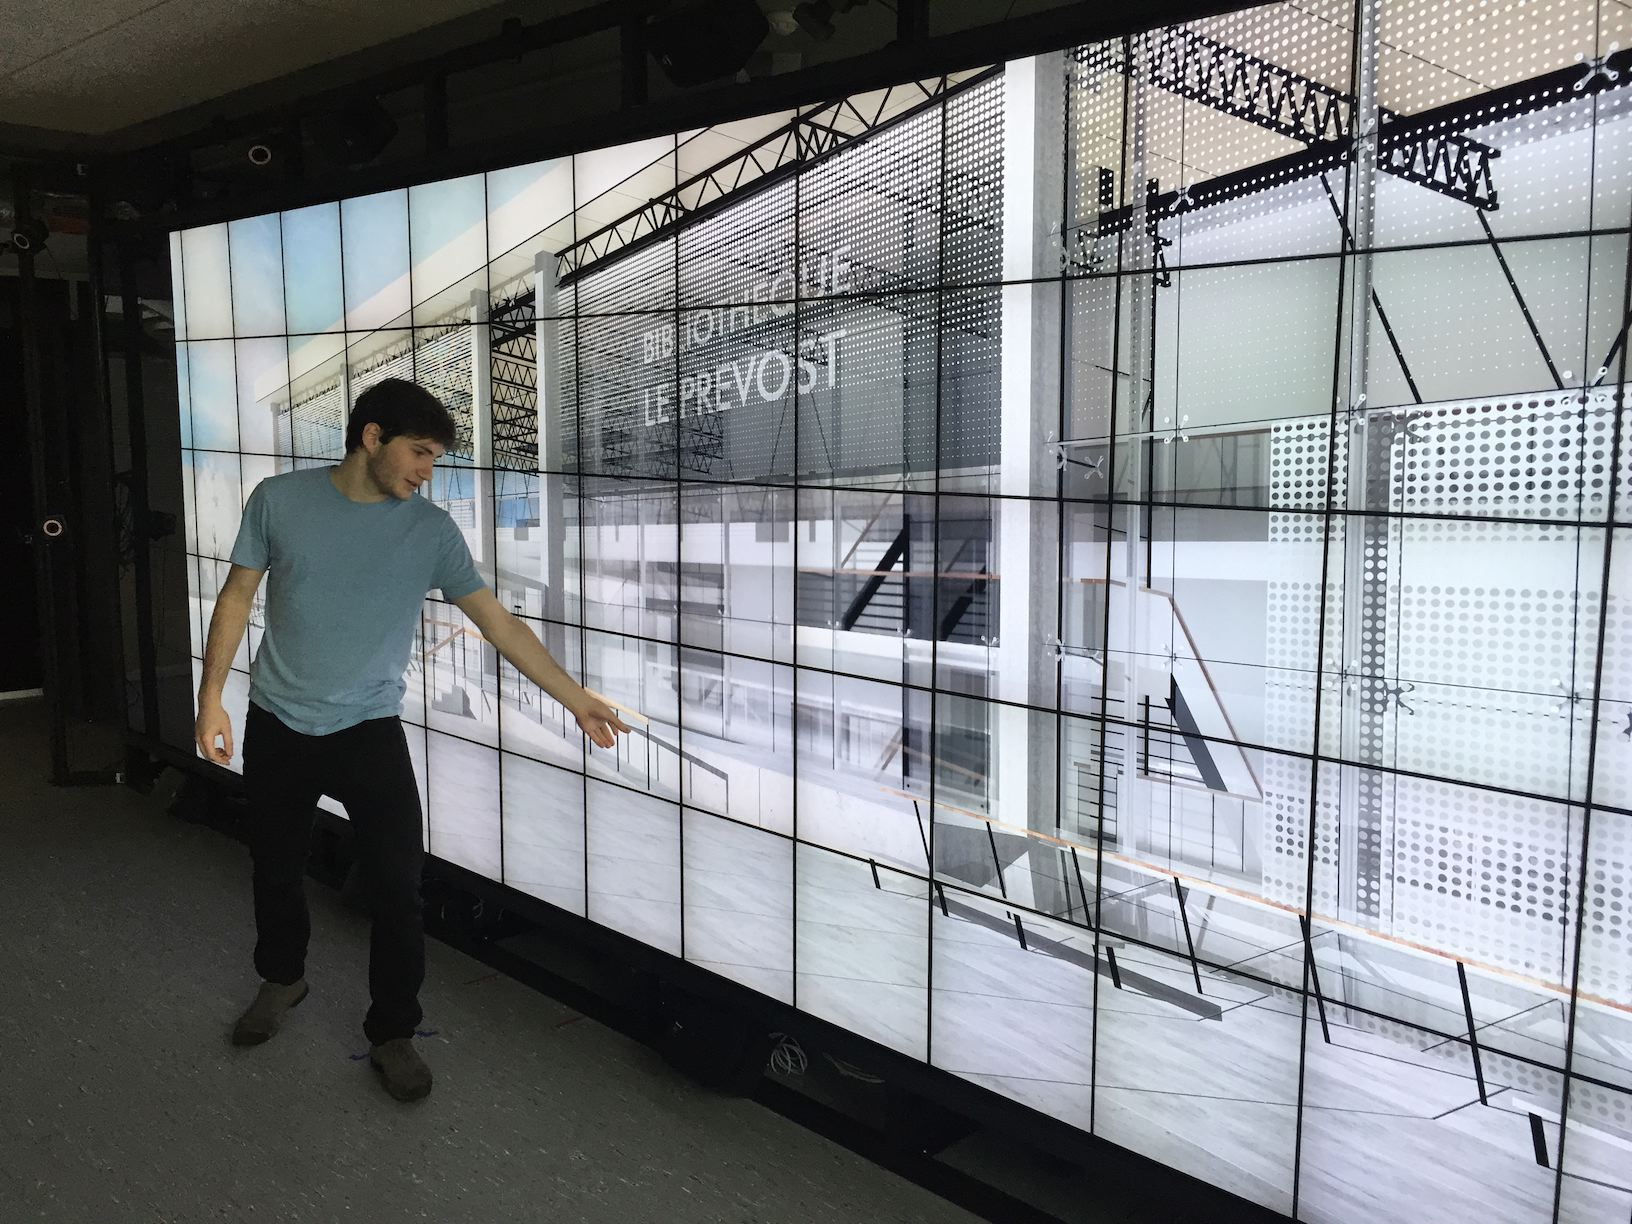
\includegraphics[height=3.3cm]{figures/ch1/wilder}
    \caption{Large image wall composed of high resolution touch screens (WILDER, in$\lvert$situ$\rvert$, LRI).}
    \label{fig:1_vi:wall}
  \end{subfigure}
  \begin{subfigure}{.3\textwidth}
    \centering
    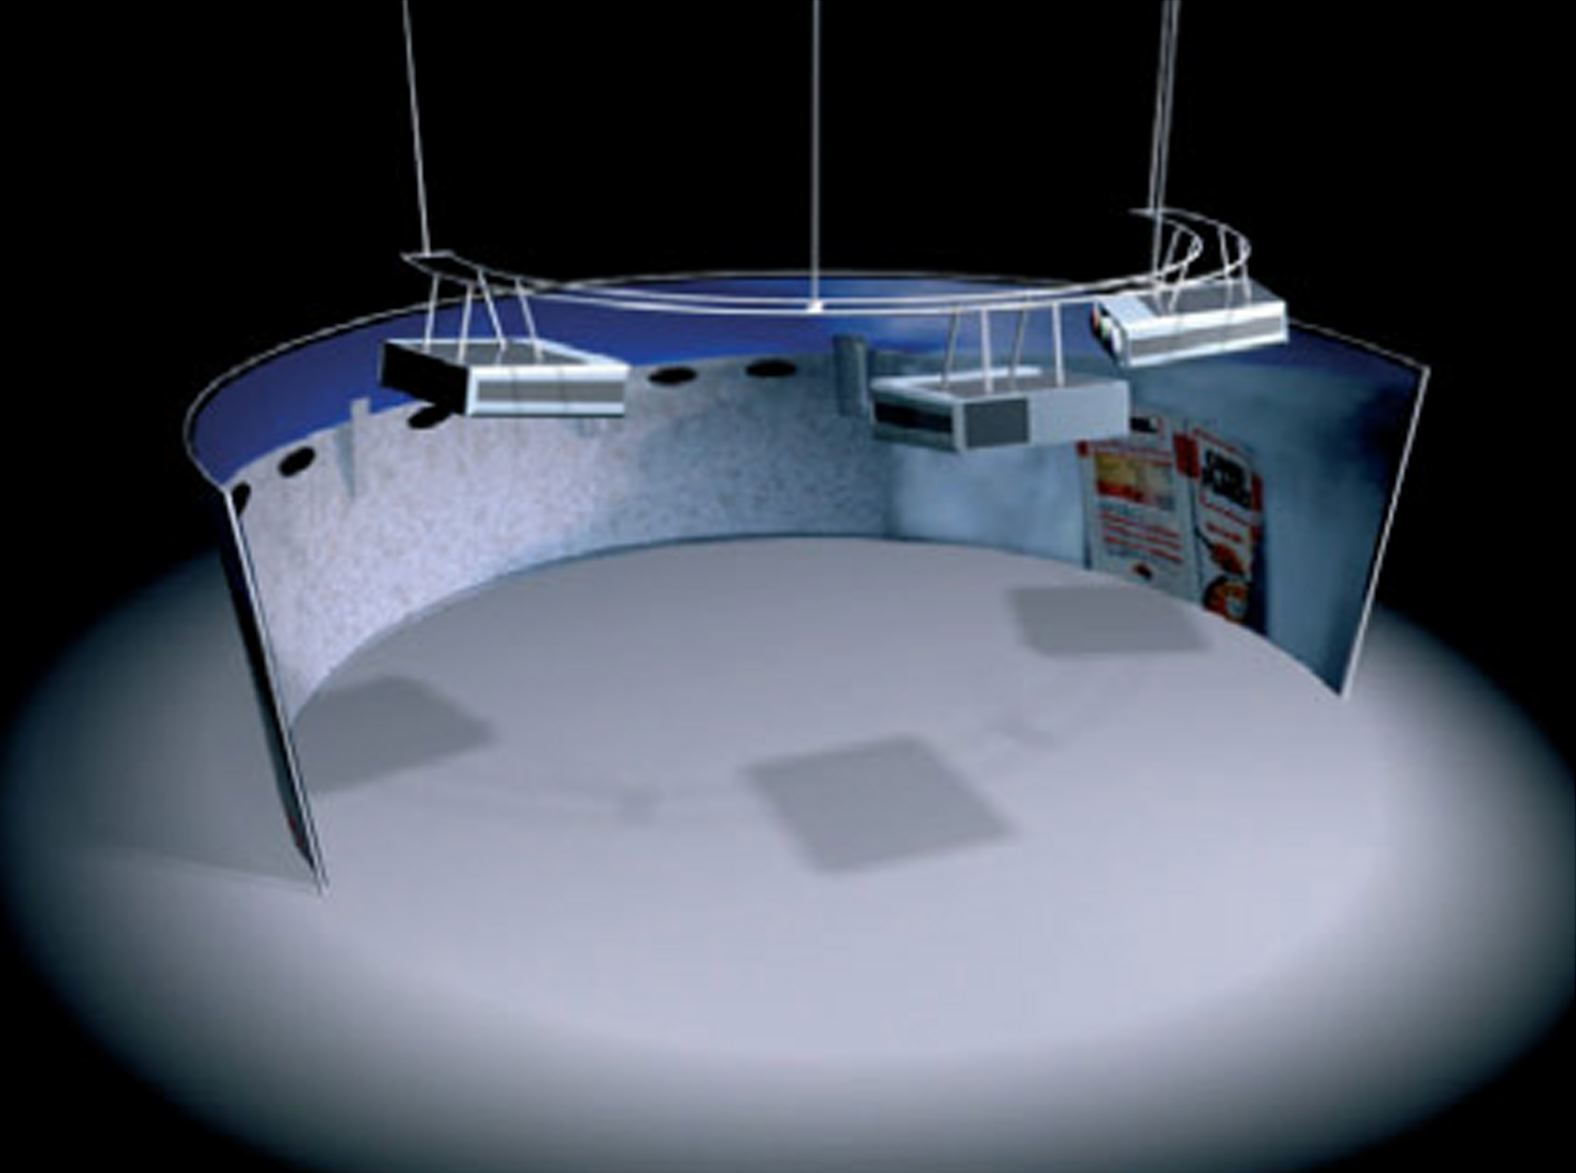
\includegraphics[height=3.5cm]{figures/ch1/icone}
    \caption{The curved panoramic projection screen i-Cone\texttrademark{} \citep{Simon2002Icone}.}
    \label{fig:1_vi:icone}
  \end{subfigure}
  \begin{subfigure}{.5\textwidth}
    \centering
    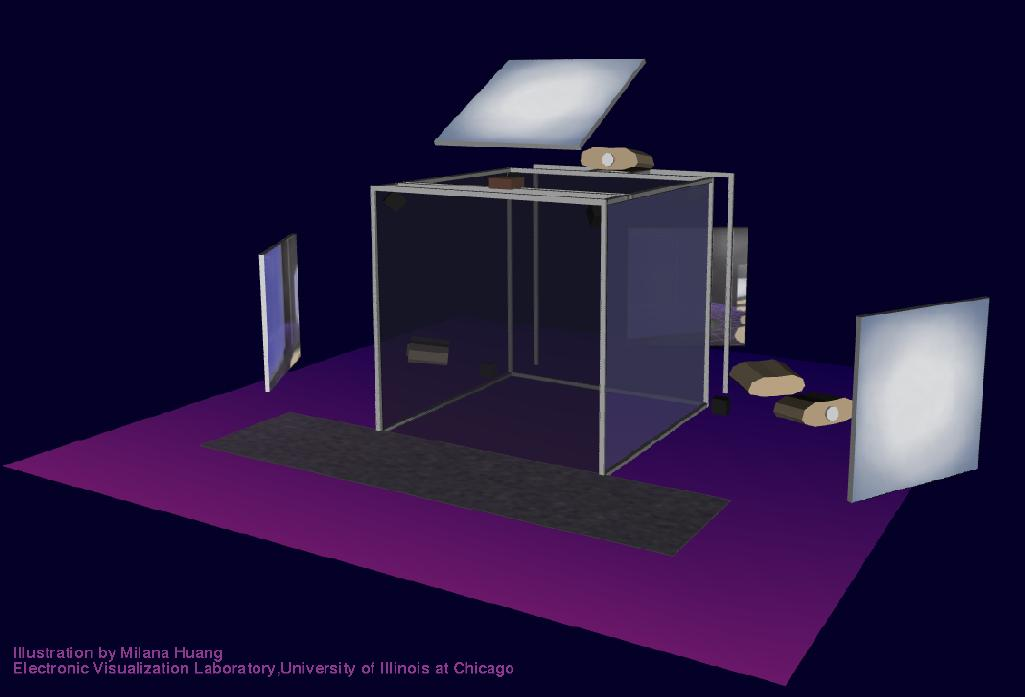
\includegraphics[width=0.9\linewidth]{figures/ch1/cave}
    \caption{CAVE\texttrademark{}: Cave Automatic Virtual Environment \citep{CruzNeira1992CAV}.}
    \label{fig:1_vi:cave}
  \end{subfigure}
  \begin{subfigure}{.45\textwidth}
    \centering
    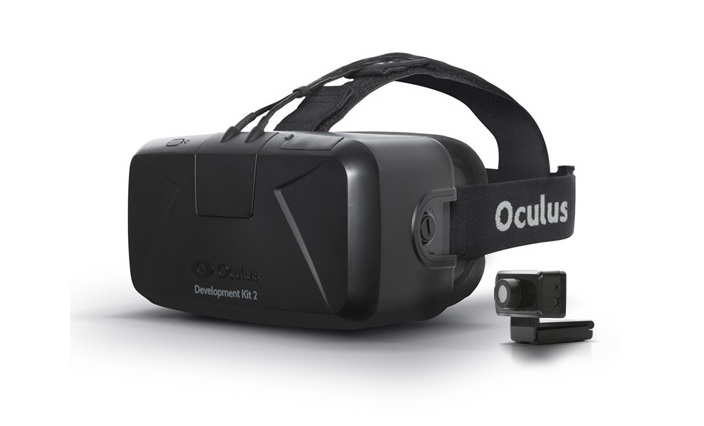
\includegraphics[width=\linewidth]{figures/ch1/oculus}
    \caption{Head-Mounted Display (HMD): Oculus DK2 \copyright{} Oculus VR LLC.}
    \label{fig:1_vi:hmd}
  \end{subfigure}
  
  \caption{\label{fig:1_vi}Different types of visual interfaces.}
\end{figure}


\subsubsection{Audio Interface}
Audio cues are very important for us to perceive events happen in the real world, similarly, the virtual world would be much less appealing if there is no sound. A virtual object would be more ``realistic" if there is a corresponding spatialized sound combined with its visual representation displayed in stereoscopy. For example, a virtual telephone displayed in front of a user with a ringtone coming exactly from that location would make the user believe that the telephone is ringing. A virtual environment filled with ambiance noises and spatialized sound coming from different virtual entities can enhance user's feeling of ``being in that world".

Audio interface has two types of roles: (1) to capture and transfer the sound made by the user (speech, hand clapping, etc.) to the computer system; (2) to transfer audio stimuli from the virtual environment (and from other users connected to the same VE) to the user. The implementation of binaural audio interface managing spatialized sound requires quite complex hardware and software setup which involves lots of research and engineering efforts \citep{Begault1994Sound}. Currently two solutions exist: first, based on Head-Related Transfer Function (HRTF) \citep{Kistler1992HRTF} which is a response that characterizes how an ear receives a sound from a point in space, a binaural sound can be reproduced using a stereo headphone combined with head tracking for one user; second, we can use a group of loudspeakers to reproduce physically the acoustic field based on Wave Field Synthesis \citep{Verheijen1998WFS}, which is independent with listener's position. The first solution is more portable and light-weight while the second is more suitable for large acoustic rooms or theaters.


\subsubsection{Haptic Interface}
The word \textit{haptic} coming from Greek means ``pertaining to the sense of touch". Haptic technology was first developed for tele-operation task so that users can enhance the remote control of machines and devices. Now more and more virtual reality applications integrate haptic interface so users can ``tele-operate" objects in the virtual world. With the help of haptic feedback, users can not only perceive virtual objects' different properties (shape and texture, etc.) by touch, but also interact physically with them (e.g. to push a virtual forklift \citep{Martin2012Forklift}). Being able to imply the sense of touch in the interaction within virtual environment is a huge step forward in aim of creating fully immersive experience in the virtual world, though lots of technical issues remain to be solved. 

Generally speaking, haptic technology aims to recreate the sense of touch by applying two kinds of stimuli to the user: tactile feedback and proprioception feedback. Tactile sensation is formed from several modalities including pressure, skin stretch, vibration and temperature, while proprioception feedback concerns the feeling of having physical contact between different parts of human body and the virtual environment. Many haptic devices on the market provide force feedback and vibration for part of the human body, especially the hands and arms, for example, electromechanical haptic arms shown from Figure~\ref{fig:1_hi:phantom} to \ref{fig:1_hi:scale1} have different workspace size and accessible force range to provide from desktop-based to room-sized haptic interaction. Some glove-shaped (Figure~\ref{fig:1_hi:dexmo}) or string-based (Figure~\ref{fig:1_hi:spidar}) devices equipped with finger-level motors can support even finer force feedback to the user for actions like object grasping and manipulating with fingers. However, there seems still no easy solution to provide full-body haptic feedback and tactile experience with relatively complex objects, so sometimes real objects (called props or tangible interfaces) are introduced into the virtual environment for passive haptic feedback in specific applications (Figure~\ref{fig:1_hi:prop}).

\begin{figure}[htb]
  \begin{subfigure}{.3\textwidth}
    \centering
    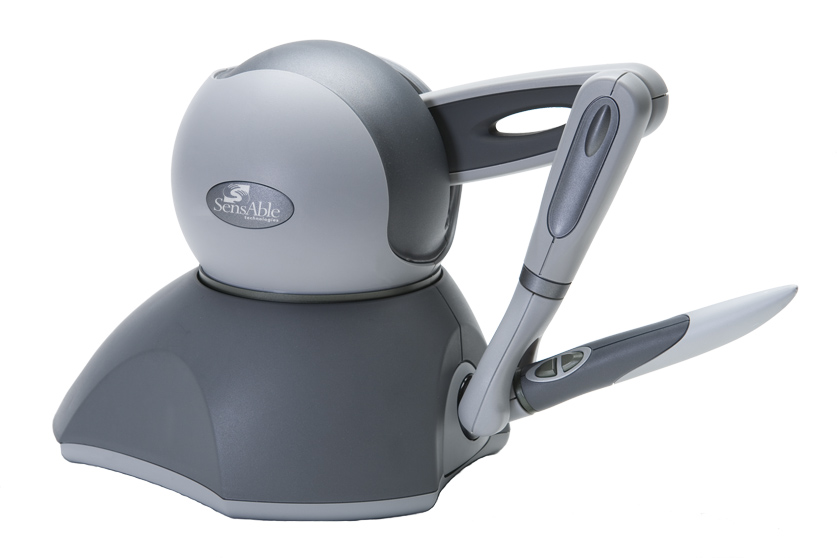
\includegraphics[width=0.8\linewidth]{figures/ch1/phantom}
    \caption{PHANTOM\textregistered{} Omni haptic arm \copyright{} Sensable.}
    \label{fig:1_hi:phantom}
  \end{subfigure}
  \begin{subfigure}{.3\textwidth}
    \centering
    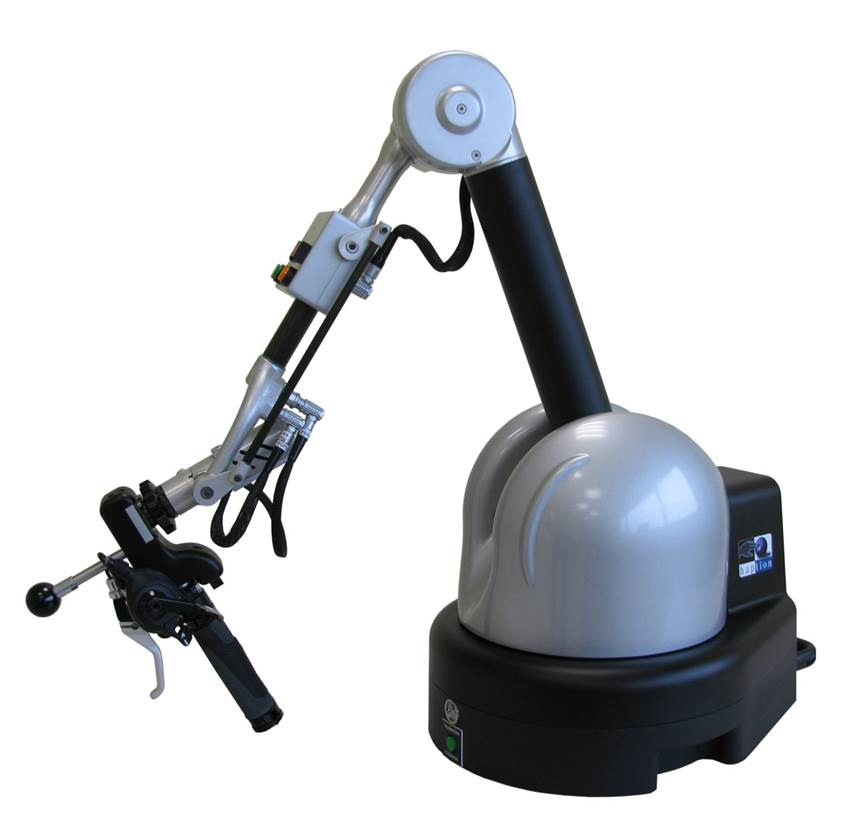
\includegraphics[width=0.8\linewidth]{figures/ch1/virtuose}
    \caption{The Virtuose 6D haptic arm \copyright{} Haption.}
    \label{fig:1_hi:virtuose}
  \end{subfigure}
  \begin{subfigure}{.35\textwidth}
    \centering
    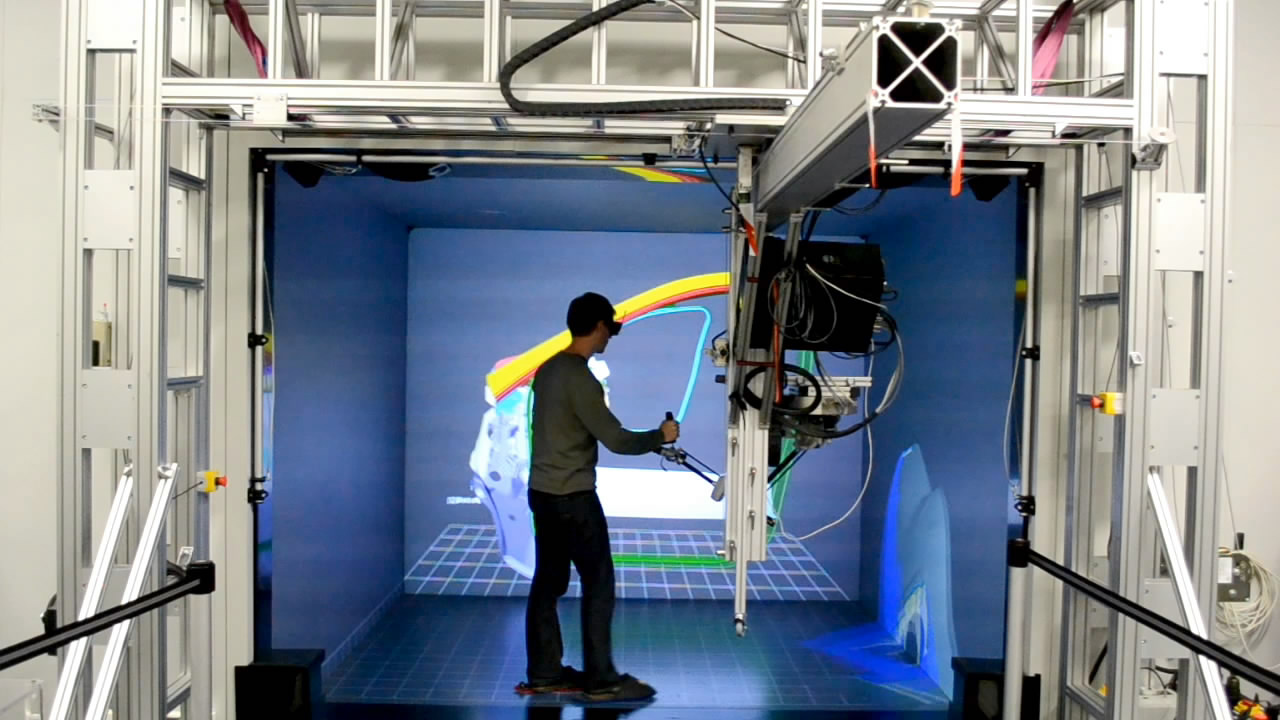
\includegraphics[width=0.9\linewidth]{figures/ch1/scale1}
    \caption{Scale one room-sized haptic solution \copyright{} Haption.}
    \label{fig:1_hi:scale1}
  \end{subfigure}
  \begin{subfigure}{.3\textwidth}
    \centering
    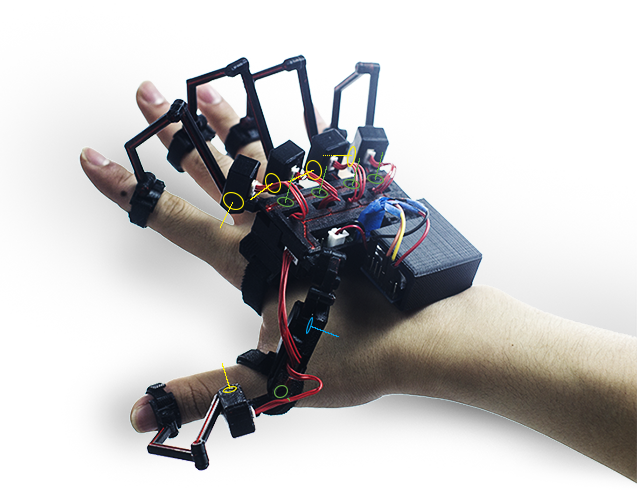
\includegraphics[width=\linewidth]{figures/ch1/dexmo}
    \caption{Dexmo\textregistered{} wearable mechanical exoskeleton \copyright{} Dexta Robotics.}
    \label{fig:1_hi:dexmo}
  \end{subfigure} 
  \begin{subfigure}{.35\textwidth}
    \centering
    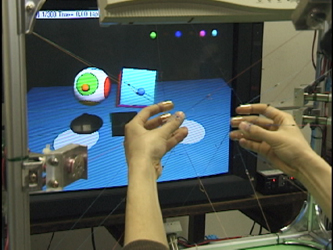
\includegraphics[width=0.9\linewidth]{figures/ch1/spidar}
    \caption{SPIDAR: string-based force feedback device \citep{Sato2002SPIDAR}.}
    \label{fig:1_hi:spidar}
  \end{subfigure}
  \begin{subfigure}{.32\textwidth}
    \centering
    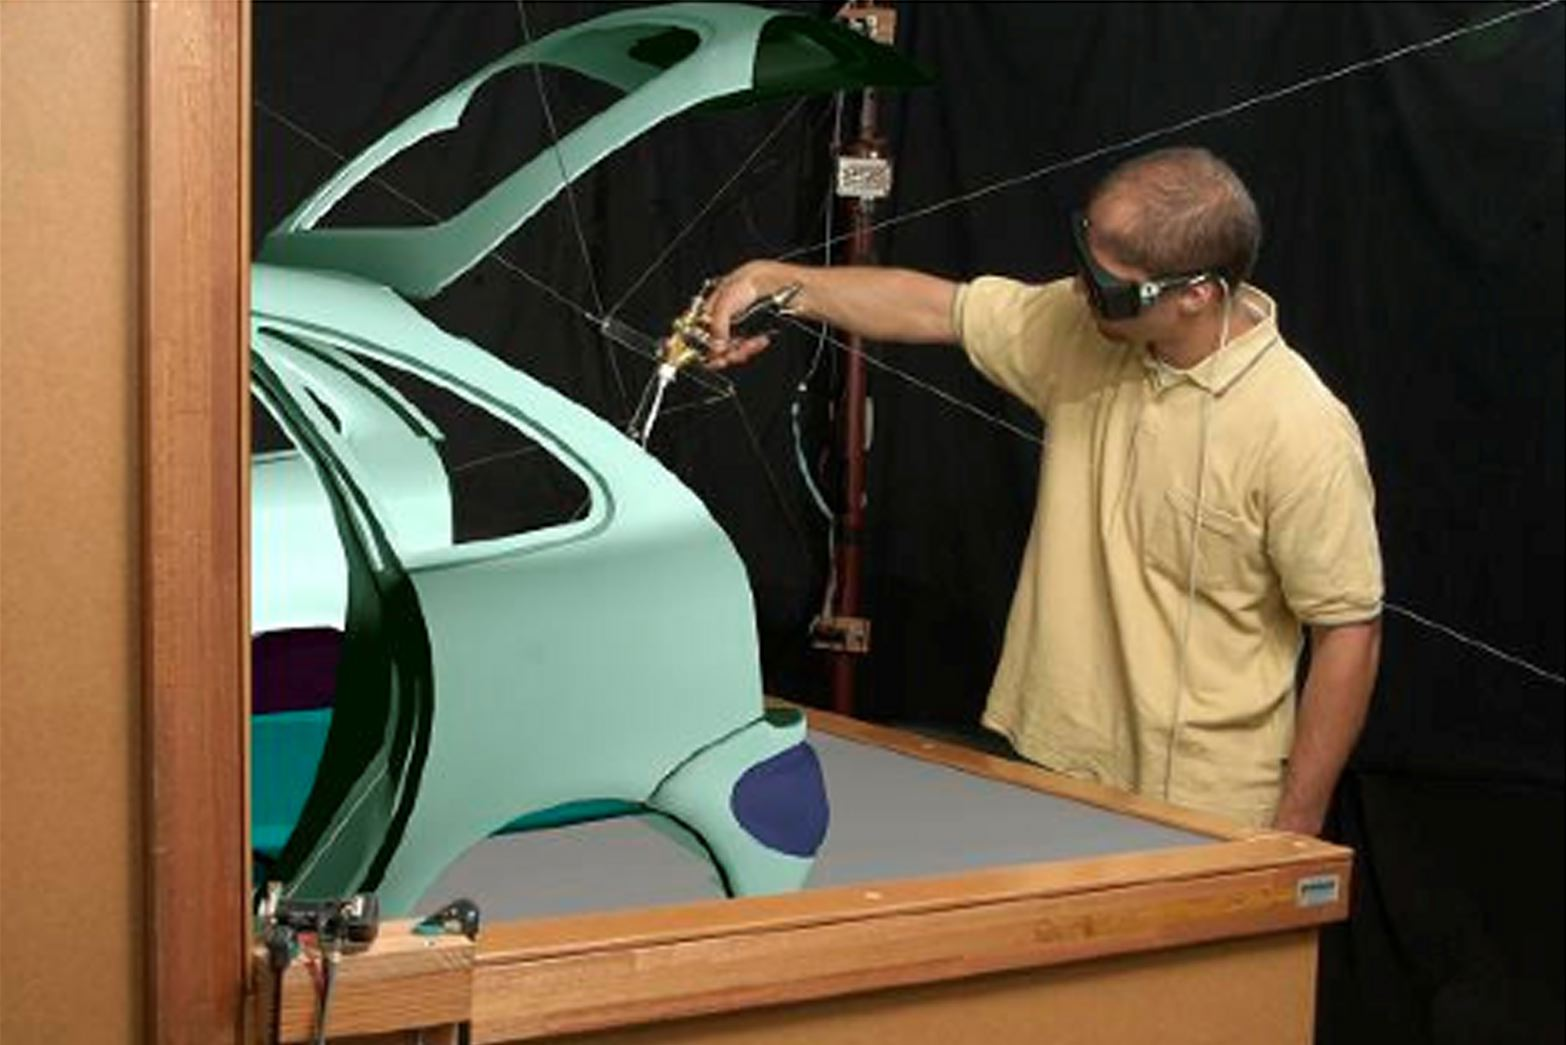
\includegraphics[width=0.9\linewidth]{figures/ch1/prop}
    \caption{The putty gun served as prop offering passive haptic feedback \citep{Ortega2005Prop}.}
    \label{fig:1_hi:prop}
  \end{subfigure}
  \caption{\label{fig:1_hi}Different types of haptic interfaces.}
\end{figure}

\subsubsection{Tracking Interface}
\label{sec:tracking}
The goal of tracking interface is to capture and transfer user's motor information as input for the computer system to update the virtual world and to generate proper sensorial stimuli (visual, audio, etc.) for the user. Tracking an entity in 3D space requires six degrees of freedom (DoF) information: three for position in form of a vector $(x, y, z)$ and three for orientation in form of Euler angle $(\theta{x},\theta{y},\theta{z})$.

In many virtual reality applications, it is sufficient to track user's head and dominant hand to respectively ensure correct visual rendering according to user's viewpoint and to allow basic interaction (e.g. object selection) in the virtual world. However, full-body movement tracking (motion capture) is increasingly demanded to enrich interaction scenarios and to enhance the level of immersion. Moreover, when multiple users are inside the same virtual environment, full-body tracking combined with decent avatar representations largely facilitate social human communication (which will be further discussed in section~\ref{sec:user-com}) by transferring subtle non-verbal cues (postures and gestures) among users. Recently, eye tracking technology has received a lot of attentions for its potential benefits in many domains \citep{Duchowski2007Eye} and it will become an important part of tracking interface for virtual reality systems.

Tracking interface can be implemented with different physical principals, including mechanical, electromagnetic, optical or acoustic methods \citep{Meyer1992Survey}. Although no single technology works for all purposes, certain methods work quite well for specific applications \citep{Welch2002Survey}. The new trend now is to combine different tracking technologies into one product to get better tracking quality, e.g. the hybrid suit from ART\footnote{http://www.ar-tracking.com/products/motion-capture/hybrid-suit} is a combination of optical, mechanical and magnetic trackers. Video based tracking devices using computer vision methods, such as kinect and leap motion (Figure~\ref{fig:1_video_tracking}), are also getting more popular because of their low cost and easy setup procedure.


\begin{figure}[htb]
  \begin{subfigure}{.5\textwidth}
    \centering
    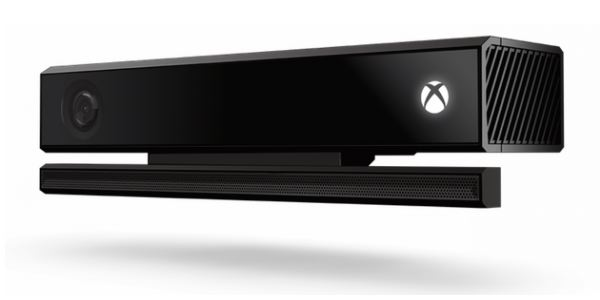
\includegraphics[height=3cm]{figures/ch1/kinect}
    \caption{The Kinect (version 2) \copyright{} Microsoft.}
    \label{fig:1_video_tracking:kinect}
  \end{subfigure}
  \begin{subfigure}{.5\textwidth}
    \centering
    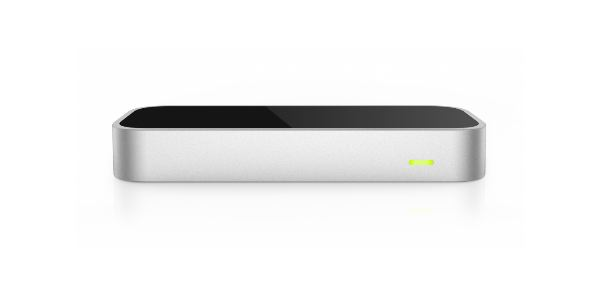
\includegraphics[height=3cm]{figures/ch1/leap}
    \caption{Leap motion controller \copyright{} Leap Motion.}
    \label{fig:1_video_tracking:leap}
  \end{subfigure}
  \caption{\label{fig:1_video_tracking}Video-based tracking interfaces.}
\end{figure}

\subsubsection{Other Interfaces}
Apart from major sensory channels like vision, audio and the sense of touch, the human sensorimotor system is way more complex and all senses could contribute to the feeling of presence in the virtual world. For example, \citet{Matsukura2011MSF} designed a multi-sensorial field (MSF) display which can generate air flow and odor vapors to simulate odor distribution in the virtual world, and \citet{Narumi2011Flavors} developed a ``Pseudo-gustation" method to change the perceived taste of food by changing its appearance and scent. However, integrating all types of behavioral interfaces into a single virtual environment remains a challenge because of the complexity and compatibility issues of different hardware and software solutions. 


\subsection{Human in Virtual Environment}
As we discussed before, virtual reality is a human-centered research domain. Technical advancement concerning the modeling of virtual world and the design of behavioral interfaces all serve to provide a better feeling of ``being in another world" (presence) for the human in virtual environment. So to understand human activity and sensation at perceptual and cognitive levels is a key to the success of virtual reality system.

\subsubsection{3D Interaction}
The interaction between the user and 3D virtual world begins once he/she is inside the virtual environment, and these human activities can be divided into some basic behaviors named Virtual Behavioral Primitives (VBP) \citet{Fuchs2011Book}. VBPs can be grouped into five categories:

\begin{itemize}
  \item observation;
  \item moving;
  \item acting;
  \item communicating with others;
  \item application control.
\end{itemize}

In the list above, except for application control, these activities are the same that people practice in the real world. Observation is our first triggered action after we dived into a virtual environment, which is a relatively passive action. The only interaction part is that when user turns head or has ocular movements (captured with eye tracking), the system will adapt the visual and audio rendering accordingly. Moving or navigation in the virtual world is also a basic interaction for the user to accomplish various tasks like object searching or transporting, way finding, sightseeing, etc. Besides natural walking, many virtual navigation metaphors are developed to effectuate more efficient virtual viewpoint control under different specific conditions (more details to be presented in Chapter \ref{chapter:nav_cohab}). Regarding ``acting", which is a vague notion, is further broke into object selection, manipulation and symbolic input by \citet{Bowman2004UIT}. The way we interact with virtual object is still quite different than with real objects due to technical limitations (e.g. lack of detailed and robust haptic feedback), thus many interaction metaphors are proposed to enable other forms of interaction \citep{Hand1997Survey}.

When interacting in an immersive virtual environment, user's sensory channels are partly blocked by the computer system. However, this does not change the fact that the user is still in the real world, thus he/she is constrained by limits of the physical workspace, for example, the user can not cross real walls or screen displays. The implication of these real world constrains on the use of immersive virtual environment is a major issue of this manuscript and will be discussed in Chapter \ref{chapter:nav_cohab}).


\subsubsection{Presence}
Sensorial immersion offered by immersive virtual environment can give user the illusion of ``being there" or the feeling of presence \citep{Heeter1992Presence}, which is a central concept of virtual reality. Presence, or telepresence, is used to describe user's subjective feeling of being immersed in a virtual environment, while the term ``immersion" is a product of technology that facilitates the production of multimodal sensory stimuli to the user \citep{Slater1994DepthPre, Bystrom1999Model}. Presence in virtual reality is a psychological state relying on sensorimotor illusion, which is different than the presence feeling at cognitive level that we have in dreams or by reading a book.

This general definition of presence is shared by many researchers, but there are still nuances in the explanations and interpretations of the definition.

\citet{Slater1994DepthPre} suggest that presence is assessed by the subjects as their sense of ``being there", the extent to which they experienced the virtual environments as more the presenting reality than the real world in which the experiment was taking place, and the extent to which the subject experienced the virtual environments as places visited rather than images seen. Then \citet{Kim1997Telepresence} describe presence as the product of two factors: (1) ``the arrival" or the feeling of being ``there" in the virtual environment, and (2) ``the departure" or the feeling of not being there ``there" in the physical environment. ``The arrival" (or one's involvement in a virtual environment) occurs when an individual concentrates their energy and their attention onto a stimulus and the events happening in the virtual environment, thus permitting the augmentation of the degree of involvement or of presence. Similarly, \citet{Witmer1998MPV} relate presence in part to the concept of attention: presence may vary across a range of values that depends in part on the allocation of attentional resources. They think that both involvement and immersion are necessary for experiencing presence. \citet{Lombard1997Heart} have attempted to offer another explanation of the concept of presence as they define presence as the perceptual illusion of non-mediation, which focuses on the transparency of behavioral interfaces.

Studies have shown that the level of presence has not only a pronounced effect on user's task performance \citep{Dangelo2008Benefits}, but also an impact on the social relationship between collaborators \citep{Slater2000Small}. To step further towards a more complete virtual reality system which could invoke higher level of presence for the user, it is important to identify factors that contribute to the formation of presence and to establish related evaluation models. Being an ongoing research topic, existing models for presence measurement are restricted to subjective rating through questionnaires \citep{Usoh2000Using, Witmer1998MPV}. The use of physiological measures for presence evaluation has been attempted \citep{Meehan2002Physiological}, but we still need more follow-up studies to design a complete evaluation model based on physiological indicators. A detailed analysis of influencing factors of presence and a taxonomy for presence measurement methods are presented by \citet{Schuemie2001Pres}.


\subsubsection{Cybersickness}
Cybersickness is a polygenic \citep{Kennedy1992Simulator} and troublesome problem with current virtual reality technology. Cybersickness, or simulator sickness (they may be different according to \citet{Stanney1997Cybersickness}), is the tendency for some users to exhibit symptoms that parallel symptoms of classical motion sickness both during and after being immersed in virtual environments. Short-term symptoms of cybersickness have been identified after repeated studies \citep{Lawson2002Signs}, but currently we still know little about its long-term effects. It is essential to understand the causes for cybersickness and to find ways to eliminate it for better use of virtual reality technology.

Researchers have tried to identify factors that are susceptible to cause cybersickness when using a virtual environment. For example, \citet{Rich1996AICS} examined the relationship between sensory compatibility and cybersickness symptoms, while \citet{So2002Scene} emphasized that the visual complexity of the virtual scene should also be taken into consideration. Technical issues such as lags \citep{Pausch1992Literature}, flickers \citep{Harwood1987Temporal}, and individual factors like gender \citep{Biocca1992Will} and age \citep{Reason1975Motion}, all have some influences on the severity of cybersickness symptoms. A more complete list of primary factors that contribute to the cause of cybersickness was provided by \citet{LaViola2000DCV}. He also gave an interesting discussion on three conflicting theories that try to explain the occurrence of cybersickness.

Currently, to evaluate the severity of cybersickness, the Simulator Sickness Questionnaire (SSQ) \citep{Kennedy1993SSQ} remains the reference tool. SSQ groups all symptoms around three main factors: nausea (nausea, stomach awareness, etc.), oculomotor (eyestrain, blurred vision, etc.) and disorientation (dizziness, vertigo). The development of various physiological measurements also begins to show interesting correlation between cybersickness symptoms and various physiological indicators \citep{Kim2005Characteristic, Min2004Psycho, Sugita2008Quantitative}. However, further research efforts are required to establish a valid cybersickness evaluation model based on physiological indicators. The study of physiological responses of human body when exposed to virtual environment will also help us to better understand the cause of cybersickness.

\subsection{Summary}
This first part of Chapter \ref{chapter:context} gives a brief introduction of virtual reality around its three main components: virtual environment, behavioral interface and the user. Key notions like presence and cybersickness, as well as different hardware implementations of virtual reality system are presented, so they can be used directly later on in this manuscript. 

% -------------------------------------------------------------------------------------------------

\section{Computer Supported Collaboration}
Collaborative Virtual Environment (CVE) refers to a virtual environment that can be shared by participants connected by a computer (remote or local) network. A collaborative virtual environment (CVE) \citep{Benford2001CVE} enables multiple users to interact \citep{Schroeder2006Usability} and to achieve collaborative tasks \citep{Dodds2009Using} within the same virtual environment. Users can be co-located in the same place or connected remotely.

Users are connected with the virtual world through graphic embodiments called avatars.



\subsection{Groupware Typology}

\subsection{Collaborative Virtual Environment}

\subsubsection{Definition}

\subsubsection{User Representation}
Avatars or virtual humans have long been used as virtual representation of the users, or we can call it user embodiment \citep{Benford1995UEC}. Avatars can provide various important functions in a multi-user virtual environment \citep{Thalmann2001VHR}. For example, a user can get other users' positions, focus of interest and see what they are doing, etc. Users can also get a representation of self in the virtual environment by using self-avatars \citep{Lok2003Effects}, which may be especially useful when working with HMDs. Moreover, according to the task that the users need to achieve in the virtual context, social representation of self may be provided through dedicated virtual clothings and/or virtual tools. In an immersive virtual environment, avatars can play a crucial role for user interaction and communication \citep{Slater1994Body}. Users work together not only in a shared virtual world, but also in a shared social space where social human communication is conveyed by avatars \citep{Roberts2004SSH}.

Several techniques can be used to bring avatars to life. In a desktop configuration, we can use input devices like keyboards to activate predefined animations. While in an immersive virtual environment, real time motion capture systems such as Kinect or optical tracking devices are more suitable to map user's physical motion to an avatar \citep{Mohler2010Effect, Vera2011AugMir, Normand2012FBA}. Due to technology limitations or high cost, humanoid avatars do not commonly support facial expression and other subtle social cues. Another interesting method developed by \citet{Ogi2001SteAva} introduces a fully animated video avatar based on live video capture. \citet{Beck2013IGG} used a similar technique to enable interactions between multiple co-located users and a group of remote users by their avatars.

\subsubsection{User Communication}
\label{sec:user-com}
Social Human Communication

Spatial Communication (Spatial Reference Frame)

\subsubsection{User Interface}
\paragraph{Co-manipulation}
\paragraph{Co-navigation}

\subsubsection{From Presence to Co-presence}



\subsection{Technical Issues}
Collaborative Virtual Environment

Network Architecture, Scene Management, Data Distribution

\subsection{Summary}


\section{Conclusion}

